\chapter{Convolutional Neural Network}
\textbf{CNNs} are particular types of neural network feed forward. Their goal 
is to use multiple layers, stacked one on top of the other, in order to 
extract input-related features. These stages are organized in a hierarchical 
way, where the highest level calculates more global, more invariant features.

Unlike the networks seen so far, CNNs organize weights using 3 dimensions. From 
this point on, we will talk about the weights also considering the volume. We are 
talking of volumes because we have image width different number of channel in input,
each neuron applies as filter on all spatial dimensions and all channel. In output 
of each layer we have another volume with a deph dependant by the number of neuorns
of hidden layer. 


\begin{figure}[!ht]
    \centering
    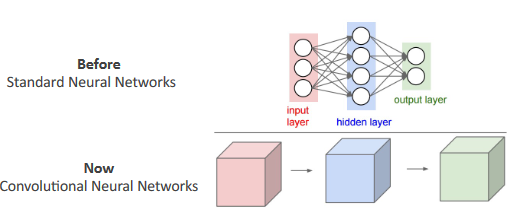
\includegraphics[width=0.5\textwidth]{img/CNN/weights.png}
    \caption{Weights representation in Feed Forward vs CNN.}
    \label{fig:weights}
\end{figure}

This particular type of network is widely used in the field of digital signal 
processing, such as image or audio signals. If we look at image processing, this 
kind of neural network offers a much more cost-effective approach than traditional 
feed forward. 

The biggest difference is related to the fact that in a feed network farward each 
input neuron is connected to all the neuorns of the next layer, this results in a 
big problem at the level of complexity, If we have an image of $100 \times 100$ pixels, 
for example, the network input is a vector of $10000$ pixels. Using CNNs means that 
each neuron is focused on a small portion of the image for each channel (\textbf{Local connectivity}) 
so that the number of neurons and connections that are created is greatly reduced.
If the image is a $1000\times 1000\times 3$, so we can have a neuron of $5\times 5 \times 3$
parameter because it applies to a path of $5\times 5$ for each deaph of the layer 
before (\textbf{full in depth}). 

\begin{figure}[!ht]
    \centering
    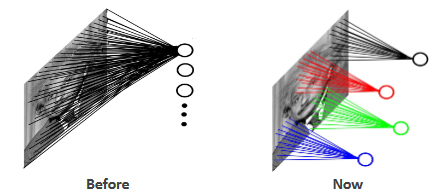
\includegraphics[width=0.5\linewidth]{img/CNN/localConn.png}
    \caption{Difference between the connections of neurons in a feed forward network and a CNN.}
    \label{fig:localConn}
\end{figure}

Also, another difference is that now, we have neurons organized in depth, we have 
multiple neurons all looking the same region of the input volume, stacked along depth.

\begin{figure}[!ht]
    \centering
    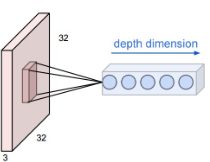
\includegraphics[width=0.25\linewidth]{img/CNN/depth.png}
    \caption{Organization of neurons in CNN}
    \label{fig:depth}
\end{figure}

In total we have $5\times 5\times 3$ weights to Learn
shared between each patch of the image, this reduce a lot the number of learning 
parameter compared to FF.  
This concept is called \textbf{weights sharing}, which means that the weights 
in the layer are shared across spatial positions. 

In general, the structure of a CNN is organized so that it has a first part, which 
includes both convolutional layers and feed forward layers, extract the main 
characteristics from the input. There is then a second part which performs the actual
classification task. We can then represent this type of network with a structure like 
the one shown in figure \ref{fig:cnn-arc}.

\begin{figure}[!ht]
    \centering
    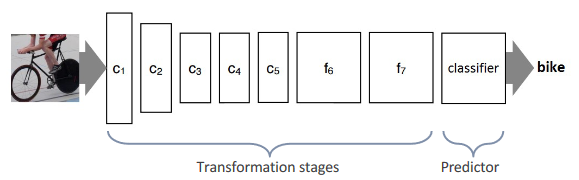
\includegraphics[width=\linewidth]{img/CNN/CNNarc.png}
    \caption{Overall CNN architecture.}
    \label{fig:cnn-arc}
\end{figure}

The concept of backpropagation can still be utilized with this architecture, which is 
very important.

Respect to traditional Neural Networks, CNNs have other special layers such as \textbf{Spatial pooling} and \textbf{Local response normalization}. These layers are 
useful to reduce computational burden, increase invariance and ease the optimization.
\section{CNNs components}
\subsection{Linear Convolution}
We begin by introducing the concept behind convolutional networks, namely the concept 
of \textbf{linear convolution}. Convolution is a linear (the operation is linear), 
local (it applies on patches) and translation-invariant
operator. If you want a richer representation of the data, you use a \textbf{filter bank},
that is a collection of $Q$ sets of $K$ filters that allows to produce an output of 
$Q$ channel.

Let's see now, on a more mathematical level, what convolution represents. First we 
introduce what we need:
\begin{itemize}
    \item $x = H \times W \times K$ is our input where $H$ represents the height dimension, $W$ the width dimension and $K$ the number of channels.
    \item $F = H' \times W' \times K \times Q$ is our filter bank where $Q$ is the number of filters that need to be apply to each channel.
    \item $y = (H - H' + 1) \times (W - W' + 1) \times Q$ is our output.
\end{itemize}

In addition to these, another very important thing to define is the \textbf{stride}. 
It represents how much I have to move my filter before I can apply it again. By default 
it is set to 1, which means I only move the center of my filter one pixel. 

\begin{note}
    16 filtri di K deph nella filter bank => 16 channel in output
\end{note}

The convolution is expressed by the following formula:
\begin{equation}
    y_{i, j, q} = y_q + \sum_{u = 0}^{H - 1}\sum_{v = 0}^{W - 1}\sum_{k = 1}^{K} x_{u + i, v + j, k} \cdot F_{u, v, k, q} 
\end{equation}

where:
\begin{itemize}
    \item $y_q$ is the bias of the filter $F_q$
    \item $x_{u + i, v + j, k}$ is the input patch of channel $k$
    \item $F_{u, v, k, q}$ is the filter for the channel $k$ that computes output channel $q$ 
\end{itemize}

\begin{figure}[!ht]
    \centering
    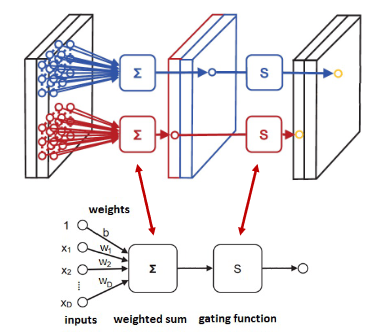
\includegraphics[width=0.5\linewidth]{img/CNN/Conv2Filter.png}
    \caption{Example of convolutional network with a filter bank of two elements.}
    \label{fig:conv2filter}
\end{figure}

We can apply filters in 2 way:
\begin{itemize}
    \item \textbf{lattice structure}: a single filter is applied to a single channel  $K=1$
    \item \textbf{multiple feature structure}: a single filter is applied to all 
    channel of the input image.$K>1$
\end{itemize}

In CNN, after appling filter we apply non linear activation function:
\begin{itemize}
    \item sigmoid
    \item tanh
    \item ReLU
    \item SmoothReLU
\end{itemize}  
activation function are called \textbf{gating function}.

\subsection{Spatial pooling}
We have already said that there are different types of layers in a CNN, one of them is 
the \textbf{spatial pooling}. This layer is intended to subsample the image in order 
to reduce the spatial scale and consequently the computation, but also to aggregate 
it to obtain the translation invariance obtaining robustness to the exact spatial 
localization of the characteristics. This is done in two main ways: 
\begin{itemize}
    \item \textbf{avg pooling}: averaging the nearest 
    pixels
    $$y_{ijk} =\max \limits_p,q\in \Omega x_{pqk}$$
    \item \textbf{max pooling}: taking the maximum value from the nearest ones
    $$y_{ijk} =\text{avg}_p,q\in \Omega x_{pqk}$$
\end{itemize}

This is done channel by channel.
\subsection{Local Response Normalization}
\textbf{Local Response Normalization} layers have the objective of normalizing the 
effect of contrast to improve the network invariance in this respect. This layer 
also allows for improved optimization and sparsity (accuracy and speed).

In general, there are two ways of applying it:
\begin{itemize}
    \item \textbf{Within Channel}: operates independently on different feature channels, and also rescales each input feature basing on a local neighborhood.
    \begin{equation}
        y_{i, j, k} = x_{i, j, k} \left(k + \alpha \sum_{(u, v) \in \mathcal{N}(i, j)} x_{u, v, k}^2 \right)^{-\beta}
    \end{equation}
    \item \textbf{Across Channels}:  Operates independently at each spatial location and groups of channels. it also normalizes groups $G(k)$ of feature channels. Groups are usually defined in a sliding window manner.
    \begin{equation}
        y_{i, j, k} = x_{i, j, k} \left(k + \alpha \sum_{q \in G(k)} x_{i, j, q}^2 \right)^{-\beta}
    \end{equation}
\end{itemize}

\subsection{Input sensibility}
CNN are sensible to the input images, morover we need a lot of datas to train from 
scratch a CNN. So we have to normalize images using:
\begin{itemize}
    \item \textbf{local mean subtraction}
    \item \textbf{normalization}
\end{itemize}
to have data centered in 0. To prevent overfitting we can use:
\begin{itemize}
    \item weight decay
    \item dropout
    \item data augmentation: for example changing illuminats, flip the image, random 
    crop and a geometric distorsion.
\end{itemize}

Remember that is always better to accept new datas.



\section{CNN Architectures}
Below, we will introduce some of the most famous CNN architectures. This is done because 
the training from 0 of one of these models requires a very large amount of data and many
computational resources.
\begin{itemize}
    \item \textbf{LeNet} is one of the first model that this is first create for the mnist 
        dataset. This network take in input a gray scale image of size $32 \times 32$.
        \begin{figure}[!ht]
            \centering
            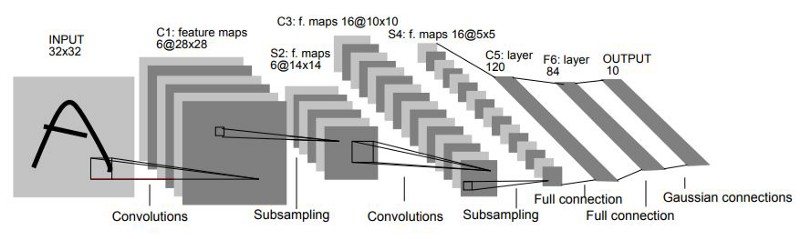
\includegraphics[width=0.5\linewidth]{img/CNN/LeNet-5.jpeg}
            \caption{LeNet}
            \label{fig:lenet}
        \end{figure}
    \item \textbf{AlexNet} was created for the imagenet challenge and combines some 
        convolutional layers with feedforward layers. It starts with a large convolutional 
        level that is gradually reduced in order to encode the deeper layers of the more 
        specific information in the task. In general we decrease filter dimension,
        increasing the depth channels
        \begin{figure}[!ht]
            \centering
            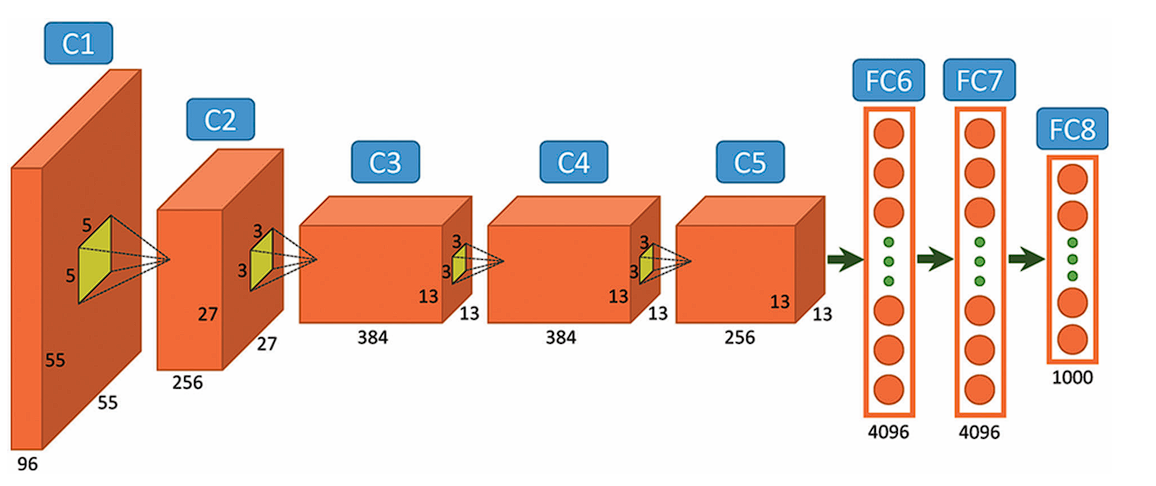
\includegraphics[width=0.5\linewidth]{img/CNN/alexNet.png}
            \caption{AlexNet}
            \label{fig:enter-label}
        \end{figure}
    \item \textbf{VGG}: is a family of CNNs that contain networks with different number of
        convolutional layers. Compared to AlexNet, they use smaller filters in order to 
        reduce the number of parameters. Also, thanks to the concept of \textbf{receptive 
            field}, if we use a smaller filter but increase the number of layers the result 
        will be the same as using a larger filter in one layer.
        \begin{figure}[!ht]
            \centering
            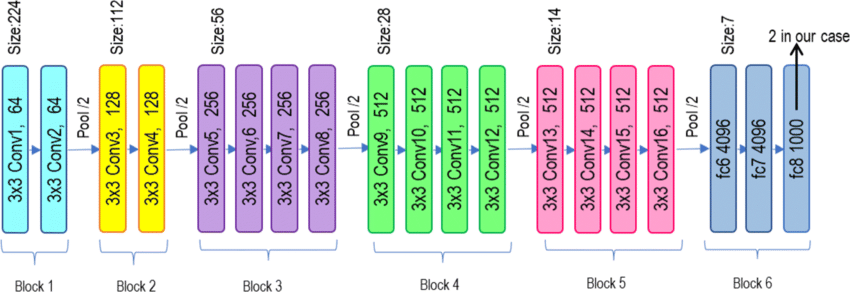
\includegraphics[width=0.5\linewidth]{img/CNN/VGG.png}
            \caption{VGG-19}
            \label{fig:enter-label}
        \end{figure}
    \item \textbf{GoogLeNet} is one of the first networks to introduce the module concept. 
        In particular, it uses the module called \textbf{inception} which is a part of the 
        network, which can be stacked over other similar modules to get a larger network. 
        As we are increasing the size of the network, we may encounter the problem of vanishing
        gradient. To solve this problem the creators introduce auxiliary output levels in 
        different parts of the network in order to inject the gradient into different levels. 
        This is done by creating a loss function which is a linear combination of the output,
        with an higher weights on final loss than the others losses.
        \begin{figure}[!ht]
            \centering
            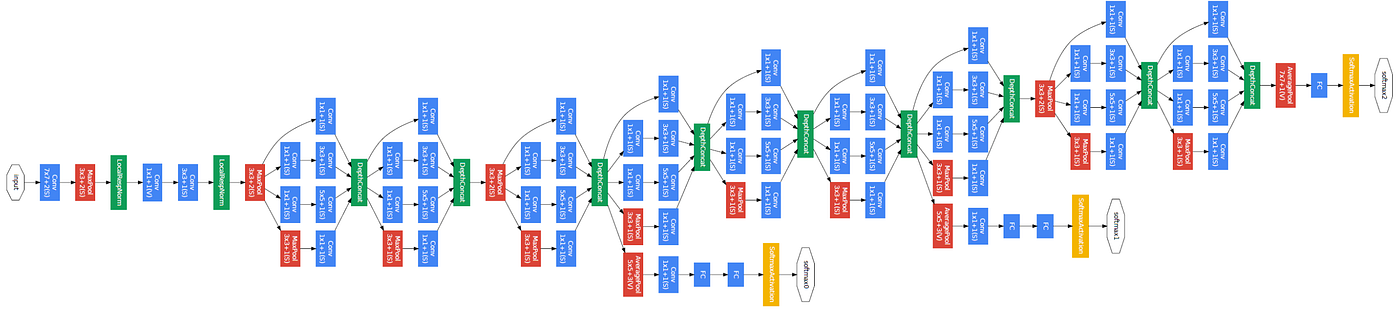
\includegraphics[width=0.5\linewidth]{img/CNN/GoogLeNet.png}
            \caption{GoogLeNet}
            \label{fig:enter-label}
        \end{figure}
    \item \textbf{ResNet} is a network type that uses the idea of residue. The basic concept is 
        to provide in input the identity function and let the network learn how to modify this 
        function to approach the one you want to learn. The identity function is used because 
        it can be easily implemented by adding the input to the result obtained at a particular 
        point in the network. This is done to limit the vanishing gradient problem as the 
        derivative of the identical function is always 1. With this trick you can implement much 
        deeper functions.
        \begin{figure}[!ht]
            \centering
            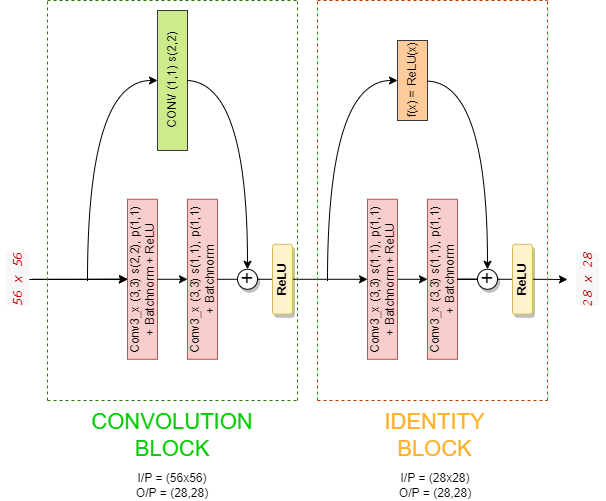
\includegraphics[width=0.5\linewidth]{img/CNN/ResNet.png}
            \caption{ResNet}
            \label{fig:enter-label}
        \end{figure}
\end{itemize}
\begin{note}
    Usually we can use $1 \times 1$ convolution to squeeze information in depth channel without 
    having impact on the spatial information.
\end{note}

\subsection{Transfert learning}
As mentioned above, it is not always possible to train a CNN from scratch. Depending on 
the situation and the amount of data available. Generally we can train model from
scratch on a big dataset, then we can finetune on our task dataset.
In general, one of the following techniques may be adopted:
\begin{itemize}
    \item New dataset is small and similar to original dataset: we can train a linear classifier 
        on CNN features from higher layers.
    \item New dataset is large and similar to original dataset: we can Fine-tune the CNN
    \item New dataset is small but very different from original dataset: we can train a linear 
        classifier on CNN features from lower layers because we have to learn general 
        features.
    \item New dataset is large and very different from original dataset: we can train CNN from 
        scratch or fine-tune it
\end{itemize}



\section{Model Compression}
When developing a DNN model, it is crucial to consider which devices it will run on, especially 
if the model is to be distributed to users. For example, it would not be practical to run an 
LLM model on a mobile device. Therefore, you need to find the right balance between performance
and compatibility. A possible solution is to keep the model in the cloud, but this choice introduces 
difficulties, such as network latency and privacy issues.

An alternative approach is to create a more compact model that can run on a mobile device and 
achieve performance similar to larger models. Another advantage of this solution is that, 
thanks to its reduced size, the inference process will be faster.

To achieve these results, several aspects were studied.
\subsection{Weight sharing}
\textbf{Weight sharing} is the simplest form of network reduction involves sharing weights between 
layers or structures within layers. Unlike other compression techniques standard weight sharing is 
carried out prior to training the original networks as opposed to compressing the model after 
training. Weight sharing reduces the network size and avoids sparsity. It is not always clear how 
many and what group of weights should be shared before there is an unacceptable performance 
degradation for a given network architecture and task.

\begin{esempio}
An example are Convolutional layers where each neuron shared weights.
\end{esempio}

\subsection{Network pruning}
Pruning weights is perhaps the most commonly used technique to reduce the number of parameters in a 
pretrained DNN. This can lead to a reduction of storage and model runtime. Performance is usually
maintained by retraining the pruned network. Iterative weight pruning prunes while retraining until 
the desired network size and/or accuracy tradeoff is met. The simplest pruning strategy involves 
setting a threshold that decides which weights or units (in this case, the absolute sum of magnitudes 
of incoming weights) are removed: threshold can both vary for each layer or be global for the whole
network. Instead of setting a threshold, one can predefine a percentage of weights to be pruned based 
on their magnitude, or a percentage aggregated by weights for each layer. Most commonly, the percentage 
of weights that are closest to 0 (in magnitude) are removed.
    
\textbf{Magnitude-based pruning} (MBP) is the most commonly used in DNNs due to its simplicity and 
performs well for a wide class of machine learning models (including DNNs) on a diverse range of tasks. 
In general, global MBP tends to outperform layer-wise MBP because there is more flexibility on the 
amount of sparsity for each layer, allowing more salient layer to be more dense while less salient 
to contain more non-zero entries.

Categorization of pruning techniques:
\begin{itemize}
    \item \textbf{Magnitude-based (iterative pruning + retraining)} pruning whereby the weights with the lowest absolute value of 
        the weight are removed based on a set threshold or percentage, layer-wise or globally.
        These are the steps:
        \begin{enumerate}
            \item Choose a neural network architecture
            \item Train the network until a reasonable solution is obtained
            \item Prune the weights of which magnitudes are less than a threshold $\tau$
            \item Train the network until a reasonable solution is obtained
            \item Iterate to step \#3
        \end{enumerate}
    \item \textbf{Methods that penalize the objective} with a regularization (L1,L2\dots) term to force the 
        model to learn a network with smaller weights and prune the smallest weights. 
        This is a pruning technique based on weight regularization, we force the 
        model's weights to be close to 0 in the objective function by adding a penalty
        term and deleting the weights closest to 0. Generally we use an L2, pay attention
        when using a regularization technique with more quadratic penalty tends to 
        too penalize larger weights.
    
    
    \item \textbf{Methods that compute the sensitivity of the loss function} when weights are 
        removed and using this as a criterion for removing weights that result in the smallest 
        change in loss. Exists differente approaches:
        \begin{itemize}
            \item \textbf{(Diagonal) Hessian-based pruning: Optimal Brain Damage}, based 
            on model compression\&speedup, it's theoretical optimal compared to current
            SOTA, but more inefficient. It delets parameters with small saliency,
            where saliency is defined by the effect on the training error. These 
            are the steps:
            \begin{enumerate}
                \item Choose a neural network architecture.
                \item Train the network until a reasonable solution is obtained.
                \item Compute the second derivatives for each parameter.
                \item Compute the saliencies for each parameter $S_k = \frac{\delta^2E}{\delta^2 u_k} u_k^2$.
                \item Sort the parameters by saliency and delete some low-saliency parameters.
                \item Iterate to step 2
            \end{enumerate}
        \end{itemize}
        
    \item \textbf{Search-based approaches} that seek to learn or adapt a set of weights to links 
        or paths within the neural network and keep those which are salient for the task.
\end{itemize}

Another important distinction to be made is that between structured and unstructured 
pruning techniques:
\begin{itemize}
    \item \textbf{Structured} aims to preserve network density for computational efficiency 
        (faster computation at the expense of less flexibility) by removing groups of weights;
    \item \textbf{Unstructured} is unconstrained to which weights or activations are removed 
        but the sparsity means that the dimensionality of the layers does not change.
\end{itemize}
Hence, sparsity in unstructured pruning techniques provide good performance at the expense 
of slower computation.

\textbf{Structured pruning via weight regularization}: Since standard pruning leads to non-
structured connectivity, structured pruning can be used to reduce memory and increase speed since 
hardware is more amenable to dealing with dense matrix multiplications, with little to no non-zero
entries in matrices and tensors. CNNs in particular are suitable for this type of pruning since 
they are made up of sparse connections.

\textbf{Group sparsity regularization}: Group sparse regularizers enforce a subset of weight 
groupings, such as filters in CNNs, to be close to zero when trained using stochastic gradient 
descent. Consider a convolutional kernel represented as a tensor $K(i; j; s; :)$, the group-wise 
$l2, 1$-norm is given as:
\begin{equation*}
    \omega_{2, 1} (K) = \lambda \sum_{i, j, s} \| \Gamma_{ijs}\| = \lambda \sum_{i, j, s} \sqrt{\sum_{t= 1}^T K(i, j, s, t)^2}
\end{equation*}
where $\Gamma_{ijs}$ is the group of kernel tensor entries $K(i; j; s; :)$ where $(i; j)$ are the 
pixel of $i$-th row and $j$-th column of the image for the $s$-th input feature map. This 
regularization term forces some $\Gamma_{ijs}$ groups to be close to zero.

\subsection{Low rank matrix and tensor decomposition} 
The idea starts from the observation that most weigths are in the fully connected layers, and that 
fully connected layers are implemented with a single matrix multiplication.
\subsection{Knowledge distillation} 
Involves learning a smaller network from a large network using supervision from the larger network and
minimizing the entropy, distance or divergence between their probabilistic estimates. Probably the 
first work about KD is from Bucilua et al. where they explored the idea of reducing model size by 
learning a student network from an ensemble of models.
\begin{itemize}
    \item They use a teacher network to label a large amount of unlabeled data and train a student 
        network using supervision from the pseudo labels provided by the teacher.
    \item They find performance is close to the original ensemble with 1000x smaller network.
\end{itemize}
    
Hinton et al. showed a neural network knowledge distillation approach where a small model is trained 
using supervision (class probability outputs) from the original “teacher” model. They showed that learning 
from the larger network outperformed the smaller network learning from scratch in the standard supervised 
classification setup.
\subsection{Quantization} 
\textbf{Quantization} is the process of representing values with a reduced number of bits. In 
neural networks, this can be applied to weights, activations and gradient values. Tipically, when 
training on the GPU, values are stored in 32-bit floating point (FP) single precision. Half-precision 
for floating point (FP-16) and integer arithmetic (INT-16) are also commonly considered. INT-16 provides
higher precision but a lower dynamic range compared to FP-16. In FP-16, the result of a multiplication 
is accumulated into a FP-32 followed by a down-conversion to return to FP-16.
    
To speed up training, faster inference and reduce bandwidth memory requirements, ongoing research 
has focused on training and performing inference with lower-precision networks using integer precision 
(IP) as low as INT-8, INT-4, INT-2 or 1 bit representations.
    
Designing such networks makes it easier to train such networks on CPUs, FPGAs, ASICs and GPUs. 
Two important features of quantization are the range of values that can be represented and the 
bit spacing.
    
For the range of signed integers with n bits, we represent a range of $[-2n-1, 2n-2]$ and for 
full precision (FP-32) the range is $\pm3.4e38$. For signed integers, there are $2n$ values in that 
range and approximately $4.2e9$ for FP-32. FP can represent a large array of distributions which is 
useful for neural network computation, however this comes at larger computational costs when compared 
to integer values.
    
For integers to be used to represent weight matrices and activations, a FP scale factor is often used 
hence many quantization approaches involve a hybrid of mostly integer formats with FP-32 scaling 
numbers. This approach is often referred to as mixed-precision (MP). Different MP strategies have 
been used to avoid overflows during training and/or inference of low resolution networks given the 
limited range of integer formats.

\subsection{Low resource and efficient architectures}
\begin{figure}[!ht]
    \centering
    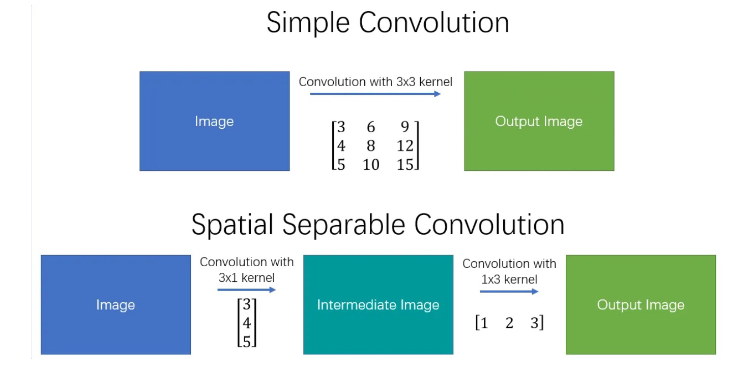
\includegraphics[width=0.5\linewidth]{img/CNN/spatialConv.png}
    \caption{Spatial Separable Convolution}
    \label{fig:spatialConv}
\end{figure}
\begin{itemize}
    \item \textbf{MobileNet}: is a sort of compression of CNN for embedded mobile vision
        application. They use depth-wise separable convolution (DSC) and 2 hyperparameters
        that trade off latency and accuracy. DSC split the convolution in 2 steps, 
        first filtering then combining outputs of each DSC filter, this is why it 
        is refered as factorization approach.
    \item \textbf{SqueezeNet}: reduce the network architecture by reducing $3\times3$ filters 
        to $1\times1$ filters (squeeze layer). Reduce the number of input channels to $3\times3$ 
        filters using squeeze layers and downsample later in the network to avoid the bottleneck of 
        information through the network too early and in turn lead to better performance. A fire module is 
        made up of the squeeze layer and an expand layer that is a mix of $1\times1$ and $3\times3$ 
        convolution filters. The number of filters per fire module is increased as it gets closer to the 
        last layer.
    \item \textbf{ShuffleNet}: uses pointwise group convolutions (i.e using a different set of 
        convolution filter groups on the same input features, this allows for model parallelization) and 
        channel shuffles (randomly shuffling helps information flow across feature channels) to reduce 
        compute while maintaining accuracy. ShuffleNet is made up economical $3\times3$ depthwise 
        convolutional filters and replace $1\times1$ layer with pointwise group convolutional followed by 
        the channel shuffle. Unlike predecessor models, ShuffleNet is efficient for smaller networks.
    \item \textbf{DenseNet}: Gradients can vanish in very deep networks because the error becomes more
        difficult to backpropogate as the number of matrix multiplications increases. DenseNets address 
        gradient vanishing connecting the feature maps of the previous layer to the inputs of the next 
        layer, similar to ResNet skip connections. This reusing of features means the network efficient 
        with its use of parameters. Although, deep and thin DenseNetworks can be parameter efficient, they 
        do tradeoff with memory/speed efficiency in comparison to shallower yet wider network because all 
        layer outputs need to be stored to perform backpropogation. However, DenseNets too can be made 
        wider and shallower to become more memory effecient if required.
\end{itemize}

